\documentclass[11pt, a4paper]{article}

% --- Packages ---
\usepackage[T1]{fontenc}
\usepackage[utf8]{inputenc}
\usepackage{mathpazo}
\usepackage[scaled=0.95]{helvet}
\usepackage{courier}
\usepackage[margin=2.5cm]{geometry}
\usepackage{amsmath, amssymb, amsthm}
\usepackage{mathtools}
\usepackage{microtype}
\usepackage{booktabs}
\usepackage{array}
\usepackage{enumitem}
\usepackage{xcolor}
\usepackage{listings}
\usepackage{hyperref}
\usepackage{cleveref}
\usepackage{tikz}
\usetikzlibrary{arrows.meta, positioning, shapes.geometric, calc}
\usepackage{stmaryrd}
\usepackage{caption}
\usepackage{subcaption}
\usepackage{titlesec}
\usepackage{abstract}
\usepackage{fancyhdr}
\usepackage{appendix}

% --- Colours ---
\definecolor{keywordcolor}{RGB}{0,0,180}
\definecolor{commentcolor}{RGB}{60,120,60}
\definecolor{stringcolor}{RGB}{160,32,32}
\definecolor{rulecolor}{RGB}{100,60,140}
\definecolor{dslcolor}{RGB}{30,80,140}
\definecolor{lightgray}{RGB}{245,245,245}
\definecolor{mygray}{RGB}{128,128,128}

% --- Listings style ---
\lstdefinestyle{bnf}{
  basicstyle=\small\ttfamily,
  backgroundcolor=\color{lightgray},
  frame=single,
  framerule=0.4pt,
  rulecolor=\color{mygray},
  breaklines=true,
  captionpos=b,
  numbers=left,
  numberstyle=\tiny\color{mygray},
  numbersep=6pt,
  tabsize=2,
  keepspaces=true,
  showstringspaces=false,
}

\lstdefinestyle{scala}{
  language=scala,
  basicstyle=\small\ttfamily,
  backgroundcolor=\color{lightgray},
  keywordstyle=\color{keywordcolor}\bfseries,
  commentstyle=\color{commentcolor}\itshape,
  stringstyle=\color{stringcolor},
  frame=single,
  framerule=0.4pt,
  rulecolor=\color{mygray},
  breaklines=true,
  captionpos=b,
  numbers=left,
  numberstyle=\tiny\color{mygray},
  numbersep=6pt,
  tabsize=2,
  keepspaces=true,
  showstringspaces=false,
  morekeywords={case, object, trait, sealed, extends, override, implicit,
                def, val, val, var, type, class, import, match, with,
                forall, exists, Set, Map, List},
}

\lstdefinestyle{dsl}{
  basicstyle=\small\ttfamily\color{dslcolor},
  backgroundcolor=\color{lightgray},
  frame=single,
  framerule=0.4pt,
  rulecolor=\color{mygray},
  breaklines=true,
  captionpos=b,
  tabsize=2,
  keepspaces=true,
}

% --- Theorem environments ---
\theoremstyle{definition}
\newtheorem{definition}{Definition}[section]
\newtheorem{example}{Example}[section]

\theoremstyle{plain}
\newtheorem{proposition}{Proposition}[section]
\newtheorem{theorem}{Theorem}[section]

\theoremstyle{remark}
\newtheorem{remark}{Remark}[section]

% --- Operators ---
\newcommand{\edges}{\operatorname{edges}}
\newcommand{\nodes}{\operatorname{nodes}}
\newcommand{\inSrc}{\operatorname{inSrc}}
\newcommand{\outTgt}{\operatorname{outTgt}}
\newcommand{\expand}{\operatorname{expand}}
\newcommand{\resolves}{\operatorname{resolves}}
\newcommand{\GNil}{\mathbf{0}}
\newcommand{\tensor}{\mathbin{*}}

% --- Header / footer ---
\pagestyle{fancy}
\fancyhf{}
\rhead{\small Graph Expansion as Concept Blending}
\lhead{\small F1R3FLY.io}
\cfoot{\thepage}
\renewcommand{\headrulewidth}{0.4pt}

% --- Hyperref ---
\hypersetup{
  colorlinks=true,
  linkcolor=rulecolor,
  citecolor=commentcolor,
  urlcolor=dslcolor,
  pdftitle={Graph Expansion as Concept Blending},
  pdfauthor={L. G. Meredith},
}

% ---
\begin{document}

\title{\textbf{Graph Expansion as Concept Blending}\\[0.5em]
  \large A Constructive Operation on Structured Graph Terms}

\author{L. G. Meredith\\
  \small F1R3FLY.io\\[0.3em]
  \small \href{mailto:lgrm@f1r3fly.io}{lgrm@f1r3fly.io}}

\date{\today}

\maketitle
\thispagestyle{fancy}

% --- Abstract ---
\begin{abstract}
We present a graph expansion operation---$\expand(G, M, F, D, S)$---that takes
a structured graph $G$ and two distinguished nodes $M$ and $F$, and produces a
new graph containing two additional nodes $D$ and $S$ whose connectivity is
defined by \emph{crossing} the port structure of $M$ and $F$. The construction
is naturally interpreted as \textbf{concept blending} in a knowledge graph: $M$
and $F$ are parent concepts, and $D$ and $S$ are the two blended offspring,
each inheriting half of each parent's relational profile in a complementary
fashion. We describe the operation in terms of a process-calculus-inspired graph
DSL, give a high-level algorithmic account, and provide a Scala implementation.
The operation exhibits a clean duality, composes well under tensor, and is
compatible with the reflective name structure of the underlying language.
\end{abstract}

\tableofcontents
\bigskip\hrule\bigskip

% ---
\section{Introduction}
\label{sec:intro}

Concept blending---the cognitive operation by which two distinct mental spaces
are selectively merged to produce a novel emergent structure~\cite{fauconnier1998}---has
long been recognized as a driver of creativity and analogical reasoning.  In
knowledge representation, blending has been modelled as a category-theoretic
pushout~\cite{goguen2005}, but practical, computable formulations that work
directly on graph structures remain less explored.

This paper proposes a concrete, graph-level blending operation grounded in a
structured graph DSL with process-calculus semantics.  Given a graph $G$ and a
pair of \emph{parent} nodes $M$ and $F$, we construct two \emph{child} nodes
$D$ and $S$ whose incoming and outgoing edges are drawn from the port sets of
$M$ and $F$ in a \emph{crossed} fashion:

\begin{itemize}[leftmargin=2em]
  \item $D$ inherits the \emph{incoming} neighbourhood of $M$ and the
    \emph{outgoing} neighbourhood of $F$.
  \item $S$ inherits the \emph{incoming} neighbourhood of $F$ and the
    \emph{outgoing} neighbourhood of $M$.
\end{itemize}

The symmetry between $D$ and $S$ is exact: swapping $M \leftrightarrow F$
simultaneously swaps $D \leftrightarrow S$, establishing a duality that mirrors
the complementary nature of blended concepts.

The remainder of the paper is structured as follows.
\Cref{sec:dsl} introduces the graph DSL and its key constructs.
\Cref{sec:algorithm} presents the expansion algorithm at a high level, together
with a worked example and a discussion of structural properties.
\Cref{sec:blending} situates the operation within the concept-blending
literature.
Appendix~\ref{app:dsl} gives a precise grammar and semantics of the DSL;
Appendix~\ref{app:scala} contains the complete Scala implementation.

% ---
\section{The Graph DSL}
\label{sec:dsl}

The graph language used throughout this paper is inspired by the
$\rho$-calculus~\cite{meredith2005}: names can be \emph{quoted graphs}, giving
the language a reflective character that is central to its expressiveness.
Below we introduce the essential constructs; a full grammar is given in
\Cref{app:dsl}.

\subsection{Core Constructs}

\begin{description}[leftmargin=2em, style=nextline]
  \item[$\GNil$] The \emph{empty graph}.  No nodes, no edges.

  \item[$v \mid G$]  \emph{Vertex introduction.}  Adds vertex $v$ to graph $G$.
    Written \lstinline[style=dsl]{v | G} in the DSL.

  \item[$G \tensor H$] \emph{Tensor product} (disjoint union).  Combines two
    graphs without identifying any nodes.  Associative and commutative up to
    isomorphism, with $\GNil$ as unit.

  \item[$(b_1,\, b_2)$] An \emph{anonymous directed edge} from the vertex
    denoted by binding $b_1$ to that of $b_2$.

  \item[$n(b_1,\, b_2)$] A \emph{named directed edge} carrying label $n$.
    Labels are \emph{names} in the DSL sense, and can themselves be quoted
    graphs: $n \;{::=}\; @G$.

  \item[\texttt{let} $x = \langle n\rangle$ \texttt{in} $G$]
    A \emph{vertex binding}: introduces a local variable $x$ standing for the
    vertex named $n$, scoped over graph $G$.

  \item[\texttt{let} $X = H$ \texttt{in} $G$]
    A \emph{subgraph binding}: introduces a local variable $X$ standing for
    subgraph $H$, scoped over $G$.

  \item[\texttt{[= G H]}] An \emph{anonymous rewrite rule} from pattern $G$ to
    replacement $H$.

  \item[\texttt{n[= G H]}] A \emph{named rewrite rule} with label $n$.
\end{description}

\subsection{Names and Reflection}

A distinctive feature of the DSL is that names can be formed by \emph{quoting}
graphs or vertices:
\[
  n \;::=\; \_ \;\mid\; x \;\mid\; X \;\mid\; @G \;\mid\; @v
\]
This means that vertices can carry structured, graph-valued names---a form of
reflection that allows the expansion operation to produce canonical names for
$D$ and $S$ (e.g., $@(M \tensor F)$ and $@(F \tensor M)$) directly from the
parent nodes.

\subsection{A Small Example}

Consider the following graph $G$ encoding a simple taxonomy:

\begin{lstlisting}[style=dsl, caption={A small graph in DSL syntax}]
let mammal = <mammal> in
let bird   = <bird>  in
let animal = <animal> in
  mammal | bird | animal | 0
  * (let x = <mammal> in x, let y = <animal> in y)
  * (let x = <bird>   in x, let y = <animal> in y)
\end{lstlisting}

Here \lstinline[style=dsl]{mammal} and \lstinline[style=dsl]{bird} are both
hyponyms of \lstinline[style=dsl]{animal}.  The expansion operation applied to
$M = \texttt{mammal}$ and $F = \texttt{bird}$ would produce two blended nodes
$D$ and $S$ that inherit crossed subsets of these taxonomic edges.

% ---
\section{The Expansion Algorithm}
\label{sec:algorithm}

\subsection{Port Sets}

\begin{definition}[Port sets]
\label{def:ports}
Let $G$ be a graph and $v$ a vertex occurring in $G$.  Define:
\begin{align*}
  \inSrc(v, G)  &\;=\; \{\, b_1 \mid (b_1, b_2) \in \edges(G),\;
                           \resolves(b_2, v) \,\}\\
  \outTgt(v, G) &\;=\; \{\, b_2 \mid (b_1, b_2) \in \edges(G),\;
                           \resolves(b_1, v) \,\}
\end{align*}
where $\resolves(b, v)$ holds when binding $b$ denotes vertex $v$ under the
ambient scoping, and $\edges(G)$ is the set of all edge pairs in $G$
(see \Cref{app:dsl} for the formal definition).
\end{definition}

Informally, $\inSrc(v, G)$ collects the \emph{sources} of all edges pointing
\emph{into} $v$, while $\outTgt(v, G)$ collects the \emph{targets} of all
edges emanating \emph{from} $v$.

\subsection{The \texorpdfstring{$\expand$}{expand} Operation}

\begin{definition}[Graph expansion]
\label{def:expand}
Let $G$ be a graph, let $M$ and $F$ be vertices of $G$, and let $D$ and $S$ be
\emph{fresh} vertices not occurring in $G$.  Define:
\[
  \expand(G, M, F, D, S) \;\coloneqq\;
    G \tensor D \tensor S
    \tensor E_D^{\mathrm{in}}
    \tensor E_D^{\mathrm{out}}
    \tensor E_S^{\mathrm{in}}
    \tensor E_S^{\mathrm{out}}
\]
where the four edge tensors are:
\begin{align*}
  E_D^{\mathrm{in}}  &= \bigotimes_{b\,\in\,\inSrc(M,G)}  (b,\, D)
  & \text{(sources of } M\text{'s in-edges point to }D\text{)}\\
  E_D^{\mathrm{out}} &= \bigotimes_{b\,\in\,\outTgt(F,G)} (D,\, b)
  & \text{(}D\text{ points to targets of }F\text{'s out-edges)}\\
  E_S^{\mathrm{in}}  &= \bigotimes_{b\,\in\,\inSrc(F,G)}  (b,\, S)
  & \text{(sources of }F\text{'s in-edges point to }S\text{)}\\
  E_S^{\mathrm{out}} &= \bigotimes_{b\,\in\,\outTgt(M,G)} (S,\, b)
  & \text{(}S\text{ points to targets of }M\text{'s out-edges)}
\end{align*}
Here $\bigotimes$ denotes iterated tensor product, with $\GNil$ as the empty
product.
\end{definition}

\Cref{fig:expansion} illustrates the crossing structure diagrammatically.

\begin{figure}[ht]
\centering
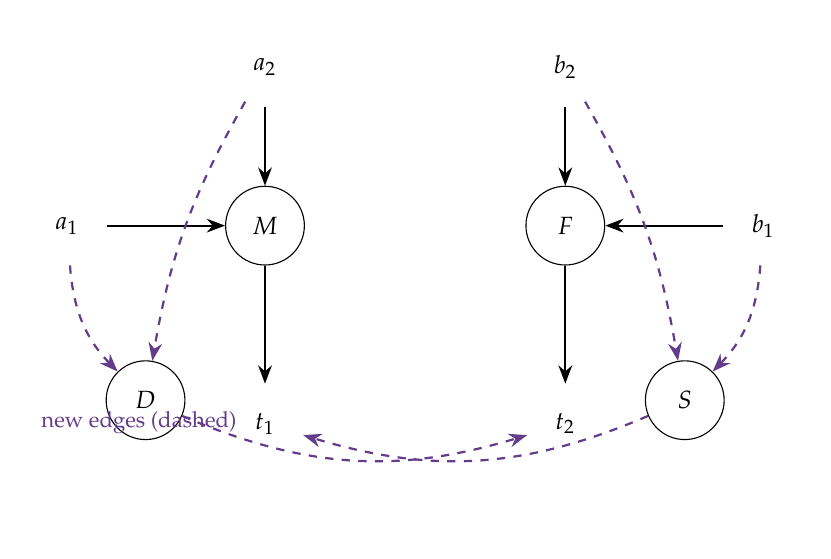
\begin{tikzpicture}[
    node distance=1.8cm and 2.8cm,
    every node/.style={draw, circle, minimum size=1.0cm, font=\small},
    arrow/.style={-Stealth, thick},
    dasharrow/.style={-Stealth, thick, dashed, color=rulecolor},
    label/.style={draw=none, font=\footnotesize\itshape},
  ]

  % Parent nodes
  \node (M) {$M$};
  \node (F) [right=of M] {$F$};

  % Child nodes
  \node (D) [below left=1.5cm and 0.8cm of M] {$D$};
  \node (S) [below right=1.5cm and 0.8cm of F] {$S$};

  % Phantom source/target nodes
  \node[draw=none] (a1) [left=1.5cm of M]  {$a_1$};
  \node[draw=none] (a2) [above=1.0cm of M] {$a_2$};
  \node[draw=none] (b1) [right=1.5cm of F] {$b_1$};
  \node[draw=none] (b2) [above=1.0cm of F] {$b_2$};
  \node[draw=none] (t1) [below=1.5cm of M] {$t_1$};
  \node[draw=none] (t2) [below=1.5cm of F] {$t_2$};

  % Original edges into M
  \draw[arrow] (a1) -- (M);
  \draw[arrow] (a2) -- (M);
  % Original edges out of M
  \draw[arrow] (M) -- (t1);
  % Original edges into F
  \draw[arrow] (b1) -- (F);
  \draw[arrow] (b2) -- (F);
  % Original edges out of F
  \draw[arrow] (F) -- (t2);

  % D: in-edges from inSrc(M), out-edges to outTgt(F)
  \draw[dasharrow] (a1) to[bend right=20] (D);
  \draw[dasharrow] (a2) to[bend right=10] (D);
  \draw[dasharrow] (D)  to[bend right=20] (t2);

  % S: in-edges from inSrc(F), out-edges to outTgt(M)
  \draw[dasharrow] (b1) to[bend left=20] (S);
  \draw[dasharrow] (b2) to[bend left=10] (S);
  \draw[dasharrow] (S)  to[bend left=20] (t1);

  % Labels
  \node[label] at ($(M)!0.5!(F)+(0,0.5)$) {};
  \node[draw=none,font=\footnotesize,color=rulecolor] at (-1.6,-2.5) {new edges (dashed)};
\end{tikzpicture}
\caption{The crossing structure of $\expand(G,M,F,D,S)$.  Solid arrows are
existing edges of $G$; dashed arrows are the new edges incident to the fresh
nodes $D$ and $S$.  Node $D$ absorbs the incoming neighbourhood of $M$ and
directs its output toward the outgoing neighbourhood of $F$; node $S$ does the
same with $M$ and $F$ swapped.}
\label{fig:expansion}
\end{figure}

\subsection{High-Level Algorithm}

The procedure is straightforward to implement:

\begin{enumerate}[leftmargin=3em]
  \item \textbf{Step 1: Collect port sets.}  Traverse $\edges(G)$ once, partitioning
    each edge $(b_1, b_2)$ into the four port sets based on whether $b_1$
    resolves to $M$ or $F$, and whether $b_2$ resolves to $M$ or $F$.

  \item \textbf{Step 2: Allocate fresh nodes.}  Choose names $D$ and $S$ not already
    present in $G$.  A canonical choice is $D = @(M \tensor F)$ and
    $S = @(F \tensor M)$ using the reflective naming of the DSL.

  \item \textbf{Step 3: Construct new edge sets.}  For each element $b$ of each port
    set, create the corresponding directed edge as per \Cref{def:expand}.

  \item \textbf{Step 4: Assemble the result.}  Return $G \tensor D \tensor S \tensor
    E_D^{\mathrm{in}} \tensor E_D^{\mathrm{out}} \tensor E_S^{\mathrm{in}}
    \tensor E_S^{\mathrm{out}}$ where the tensor is represented as a union of
    the node and edge sets.
\end{enumerate}

The algorithm runs in $O(|\edges(G)|)$ time for a single expansion, since each
edge is visited exactly once in Step~1 and the construction in Steps~3--4 is
linear in the sizes of the port sets.

\subsection{Structural Properties}

\begin{proposition}[Duality]
\label{prop:duality}
$\expand(G, M, F, D, S) \cong \expand(G, F, M, S, D)$,
where $\cong$ denotes graph isomorphism.
\end{proposition}
\begin{proof}
Swapping $M \leftrightarrow F$ exchanges $\inSrc(M,G) \leftrightarrow
\inSrc(F,G)$ and $\outTgt(M,G) \leftrightarrow \outTgt(F,G)$, which exactly
exchanges the roles of $D$ and $S$ in \Cref{def:expand}.
\end{proof}

\begin{proposition}[Self-expansion]
\label{prop:self}
When $M = F$, the nodes $D$ and $S$ produced by $\expand(G, M, M, D, S)$
receive identical port structure: $\inSrc(D) = \inSrc(S)$ and
$\outTgt(D) = \outTgt(S)$.  The expansion degenerates to adding two
isomorphic copies of a single ``self-blended'' node.
\end{proposition}

\begin{proposition}[Compositional stability]
The result of $\expand$ is a well-formed graph in the DSL as long as $D$ and
$S$ are fresh, and is itself a valid argument to a subsequent $\expand$ call.
In particular, the operation preserves the tensor-monoidal structure of the
graph category.
\end{proposition}

\begin{remark}[Labeled edges]
When edges carry labels, one may supply a label-combination function
$\omega : \mathrm{Name} \times \mathrm{Name} \to \mathrm{Name}$ to determine
how source edge labels are inherited by the new edges.  The simplest policy
preserves the label of the originating edge unchanged.
\end{remark}

% ---
\section{Concept Blending Interpretation}
\label{sec:blending}

\subsection{Blending Spaces}

In Fauconnier and Turner's theory~\cite{fauconnier1998}, a blend consists of
two \emph{input spaces} $I_1$ and $I_2$, a \emph{generic space} $G_0$
capturing shared structure, and a \emph{blended space} $B$ that selectively
projects from each input and develops emergent structure.

In our formulation:
\begin{itemize}[leftmargin=2em]
  \item The \emph{input spaces} are the local neighbourhoods of $M$ and $F$
    in $G$.
  \item The \emph{generic space} is $G$ itself, providing the ambient
    relational context.
  \item The \emph{blended spaces} are $D$ and $S$: each projects the incoming
    structure of one parent and the outgoing structure of the other, producing
    two complementary emergent entities.
\end{itemize}

\subsection{Why Two Blends?}

Classical blending produces a single blended space.  Our construction produces
\emph{two}, which are each other's mirror under the duality of
\Cref{prop:duality}.  This is reminiscent of the biological metaphor implicit
in the $M$/$F$ naming: sexual reproduction produces offspring that are distinct
but complementary recombinations of parental genetic material.  In a knowledge
graph, the two blends represent distinct \emph{conceptual stances} one can
adopt when combining $M$ and $F$: prioritising $M$'s incoming context or $F$'s
incoming context as the defining feature of the new concept.

\subsection{Knowledge Graph Applications}

The operation is directly applicable to concept graphs in which nodes are
concepts and edges are semantic relations (hypernymy, causation, parthood,
etc.).  Given two concepts $M$ and $F$:
\begin{itemize}[leftmargin=2em]
  \item $D$ is the blend that is \emph{arrived at} by the same causes/supersets
    as $M$, but \emph{leads to} the same effects/subsets as $F$.
  \item $S$ is the complementary blend: arrived at like $F$, leads to like $M$.
\end{itemize}
This provides a systematic, constructive account of creative concept formation
that is computable directly from the graph structure.

% ---
\section{Conclusion}
\label{sec:conclusion}

We have presented $\expand(G, M, F, D, S)$, a graph operation that constructs
two blended nodes by crossing the port sets of two parent nodes in a structured
graph DSL.  The operation is simple, efficient, and structurally well-behaved:
it preserves the monoidal structure of the graph category, satisfies an exact
duality, and supports a clean concept-blending interpretation.  A Scala
implementation is provided in \Cref{app:scala}.

\subsection*{Application to Categories}

Because a small category is precisely a directed graph (its \emph{underlying
graph}) equipped with a composition law and identities~\cite{maclane1998}, the
expansion operation applies directly to categories viewed as graphs.  Given a
category $\mathcal{C}$, two objects $M$ and $F$ play the role of parent nodes,
and the port sets $\inSrc(M, \mathcal{C})$ and $\outTgt(F, \mathcal{C})$ are
just the domains of morphisms into $M$ and the codomains of morphisms out of
$F$, respectively.  The blended objects $D$ and $S$ then inherit crossed
hom-set structure: the morphisms arriving at $D$ originate from the same
objects that map into $M$, while those departing from $D$ target the same
objects that $F$ maps into.  Whether $D$ and $S$ can be equipped with
composition laws that make the extended graph into a category is a non-trivial
coherence question, but the underlying graph expansion is well-defined and
meaningful regardless.

\subsection*{Quantaloids and Goertzel--Bennett Weakness}

A \emph{quantaloid} is a category enriched over the category of
quantales~\cite{rosenthal1996}: hom-sets are replaced by elements of a quantale
(a complete lattice equipped with a compatible monoid structure), and
composition distributes over arbitrary joins.  Quantaloids provide a natural
setting for reasoning about graded or uncertain relationships, and have been
proposed as a foundation for modelling cognitive uncertainty and semantic
proximity.

Goertzel has argued~\cite{goertzel2023} that Bennett's notion of
\emph{weakness}---a measure of the degree to which one pattern fails to
determine another~\cite{bennett1961}---can be captured within a quantale-based
framework, where the quantale elements represent degrees of evidential support
or causal influence.  In this setting, the hom-value $\mathcal{C}(A, B) \in Q$
(for a quantale $Q$) encodes not merely the existence of a relationship from
$A$ to $B$ but its \emph{strength} or \emph{weakness}.

The expansion operation extends naturally to this enriched setting.  The port
sets $\inSrc$ and $\outTgt$ generalise to \emph{weighted port sets}: for each
source $b$ of an edge into $M$, the edge now carries a quantale value $q \in
Q$ representing the strength of that relationship.  The blended node $D$
inherits these weighted connections, and the quantale structure determines how
weights compose along the new crossed paths.  In particular, the join operation
of $Q$ provides a canonical way to aggregate multiple weighted paths between
the same pair of nodes, while the monoid multiplication propagates weights
through composition.

We therefore conjecture that a \emph{quantaloid expansion}
$\expand_Q(G, M, F, D, S)$ is well-defined, with blended hom-values given by
\[
  Q(b,\, D) \;=\; Q(b,\, M)
  \qquad
  Q(D,\, b) \;=\; Q(F,\, b)
\]
and analogously for $S$, directly inheriting the quantale values of the parent
edges.  This would make the blending operation a morphism of quantaloid-enriched
graphs, and would ground Goertzel's weakness-based similarity judgements in a
constructive, graph-level blending procedure.  Establishing this conjecture
formally---in particular verifying the enriched composition axioms for $D$ and
$S$---is a priority for future work.

\subsection*{Further Directions}

Additional future directions include: (1) iterating the expansion to build a
\emph{blending lattice} and studying its order-theoretic properties; (2)
equipping the operation with a categorical semantics as a functor on a graph
topos; (3) integrating the construction with the Rho Calculus reduction
semantics to give blended concepts a dynamic, rewriting-based life-cycle; and
(4) applying the operation to large-scale knowledge graphs to evaluate its
utility for automated analogy and metaphor generation.

% --- References ---
\begin{thebibliography}{9}

\bibitem{fauconnier1998}
G.~Fauconnier and M.~Turner,
\textit{Conceptual Integration Networks},
Cognitive Science 22(2), 1998, pp.~133--187.

\bibitem{goguen2005}
J.~Goguen,
\textit{Mathematical Models of Cognitive Space and Time},
in \textit{Reasoning and Cognition}, Springer, 2005.

\bibitem{meredith2005}
L.~G.~Meredith and M.~Radestock,
\textit{A Reflective Higher-Order Calculus},
Electronic Notes in Theoretical Computer Science 141(5), 2005, pp.~49--67.

\bibitem{lncs2004}
L.~G.~Meredith and S.~Bjorg,
\textit{Contracts and Types},
Communications of the ACM 46(10), 2003, pp.~41--47.

\bibitem{maclane1998}
S.~Mac~Lane,
\textit{Categories for the Working Mathematician}, 2nd ed.,
Springer, 1998.

\bibitem{rosenthal1996}
K.~I.~Rosenthal,
\textit{The Theory of Quantaloids},
Addison Wesley Longman, 1996.

\bibitem{goertzel2023}
B.~Goertzel,
\textit{Generative AI and the Path to AGI: Reflections on Cognitive
Architecture and Uncertainty},
Manuscript, SingularityNET / TrueAGI, 2023.

\bibitem{bennett1961}
C.~H.~Bennett,
\textit{Logical Depth and Physical Complexity},
in \textit{The Universal Turing Machine: A Half-Century Survey},
Oxford University Press, 1988, pp.~227--257.

\end{thebibliography}

% ---
\appendix
\appendixpage
\addappheadtotoc

% ---
\section{Precise DSL Grammar and Semantics}
\label{app:dsl}

\subsection{Grammar}

The grammar below is given in LBNF (Labelled Backus--Naur Form), as used by the
BNF Converter tool.  Production labels are given before the period on each
line.

\begin{lstlisting}[style=bnf, caption={Complete LBNF grammar of the graph DSL}]
-- Coercions (precedence levels)
_ .   Graph  ::= Graph1 ;
_ .   Graph1 ::= Graph2 ;
_ .   Graph2 ::= Graph3 ;
_ .   Graph3 ::= "{" Graph "}" ;

-- Basic Graph Term Constructors
GNil .       Graph3 ::= "0" ;
GVertex .    Graph2 ::= Vertex "|" Graph1 ;
GVar .       Graph2 ::= LVar  "|" Graph1 ;
GNominate .  Graph1 ::= Binding ;
GEdgeAnon .  Graph1 ::= "(" Binding "," Binding ")" ;
GEdgeNamed . Graph1 ::= Name "(" Binding "," Binding ")" ;
GRuleAnon .  Graph1 ::= "[" "=" Graph Graph "]" ;
GRuleNamed . Graph1 ::= Name "[" "=" Graph Graph "]" ;
GSubgraph .  Graph1 ::= GraphBinding ;
GTensor .    Graph  ::= Graph "*" Graph1 ;

-- Bindings
VBind .      Binding     ::= "let" LVar "=" Vertex "in" Graph2 ;

-- Subgraph Bindings
GBind .      GraphBinding ::= "let" UVar "=" Graph "in" Graph2 ;

-- Vertices
VName .      Vertex ::= "<" Name ">" ;

-- Names
NameWildcard .    Name ::= "_" ;
NameVVar .        Name ::= LVar ;
NameGVar .        Name ::= UVar ;
NameQuoteGraph .  Name ::= "@" Graph ;
NameQuoteVertex . Name ::= "@" Vertex ;
separator Name "," ;

-- Tokens
token UVar ((upper (letter | digit | '_' | '\'')*)
           |(('_') (upper | digit | '_' | '\'')+)) ;
token LVar (((lower | '\'') (letter | digit | '_' | '\'')*)
           |(('_') (lower | digit | '_' | '\'')+)) ;

-- Comments
comment "//" ;
comment "/*" "*/" ;
\end{lstlisting}

\subsection{Precedence and Associativity}

The coercion chain $\mathtt{Graph} \succ \mathtt{Graph1} \succ \mathtt{Graph2}
\succ \mathtt{Graph3}$ encodes precedence: tensor ($*$) binds most loosely, and
braces $\{G\}$ allow any sub-expression at any precedence level.  In practice:
\[
  G * H * K \;\equiv\; (G * H) * K
  \qquad\text{(left-associative)}
\]

\subsection{Semantic Domains}

Let $\mathcal{N}$ be a countably infinite set of \emph{atoms} (ground names),
and let $\mathcal{V} = \{ \langle n \rangle \mid n \in \mathcal{N}_\infty \}$
be the set of vertices, where $\mathcal{N}_\infty$ is the closure of
$\mathcal{N}$ under quoting.

\begin{definition}[Graph denotation]
\label{def:denotation}
A \emph{graph} $G$ denotes a pair $(\nodes(G), \edges(G))$ where:
\begin{align*}
  \nodes(G) &\subseteq \mathcal{V}\\
  \edges(G) &\subseteq \mathcal{V} \times \mathcal{N}_\infty \times \mathcal{V}
\end{align*}
The edge label $*$ is used for anonymous edges; named edges carry an explicit
label from $\mathcal{N}_\infty$.
\end{definition}

The structural semantics of each construct is given in \Cref{tab:semantics}.

\begin{table}[ht]
\centering
\caption{Denotational semantics of graph DSL constructs.}
\label{tab:semantics}
\renewcommand{\arraystretch}{1.4}
\begin{tabular}{@{} l l @{}}
\toprule
\textbf{Construct} & \textbf{Denotation} \\
\midrule
$\GNil$ & $(\emptyset,\; \emptyset)$ \\
$v \mid G$ & $(\{v\} \cup \nodes(G),\; \edges(G))$ \\
$G \tensor H$ & $(\nodes(G)\cup\nodes(H),\; \edges(G)\cup\edges(H))$ \\
$(b_1,\, b_2)$ & $(\{v_1,v_2\},\; \{(v_1,*,v_2)\})$ where $v_i=\llbracket b_i\rrbracket$ \\
$n(b_1,\, b_2)$ & $(\{v_1,v_2\},\; \{(v_1,n,v_2)\})$ where $v_i=\llbracket b_i\rrbracket$ \\
$\texttt{let}\; x = v\; \texttt{in}\; G$ & substitute $x \mapsto v$ throughout $G$, return $G[v/x]$ \\
$\texttt{let}\; X = H\; \texttt{in}\; G$ & substitute $X \mapsto H$ throughout $G$, return $G[H/X]$ \\
$[{=}\; G\; H]$ & $(\emptyset,\; \emptyset)$ together with rule $G \Rightarrow H$ \\
\bottomrule
\end{tabular}
\end{table}

\subsection{The \texorpdfstring{$\edges$}{edges} Extractor}

The function $\edges$ used in \Cref{sec:algorithm} is defined recursively:

\begin{align*}
  \edges(\GNil) &= \emptyset\\
  \edges(v \mid G) &= \edges(G)\\
  \edges(G \tensor H) &= \edges(G) \cup \edges(H)\\
  \edges((b_1, b_2)) &= \{(\llbracket b_1\rrbracket,\, *,\, \llbracket b_2\rrbracket)\}\\
  \edges(n(b_1, b_2)) &= \{(\llbracket b_1\rrbracket,\, n,\, \llbracket b_2\rrbracket)\}\\
  \edges(\texttt{let}\; x = v\; \texttt{in}\; G) &= \edges(G[v/x])\\
  \edges(\texttt{let}\; X = H\; \texttt{in}\; G) &= \edges(H) \cup \edges(G[H/X])\\
  \edges([{=}\;G\;H]) &= \emptyset
\end{align*}

\subsection{Freshness and Quoting}

Two canonical fresh names for the offspring nodes are available via the
reflective quoting mechanism:
\[
  D \;\coloneqq\; \langle @(M \tensor F) \rangle
  \qquad
  S \;\coloneqq\; \langle @(F \tensor M) \rangle
\]
These are guaranteed to be distinct from any atom-named vertex in $G$, and are
themselves well-formed vertices in the DSL.

% ---
\section{Scala Implementation}
\label{app:scala}

The implementation below uses immutable case classes and pure functions.  It
targets Scala~3 and requires no external dependencies beyond the standard
library.

\begin{lstlisting}[style=scala, caption={Core graph ADT}]
// --- Names ---
enum Name:
  case Wildcard
  case VarName(id: String)
  case GraphName(id: String)     // upper-case identifier
  case QuoteGraph(g: Graph)
  case QuoteVertex(v: Vertex)

// --- Vertices ---
case class Vertex(name: Name)

// --- Bindings ---
case class Binding(varName: String, vertex: Vertex, body: Graph)

// --- Graph ADT ---
enum Graph:
  case GNil
  case GVertex(vertex: Vertex, rest: Graph)
  case GEdgeAnon(src: Binding, tgt: Binding)
  case GEdgeNamed(label: Name, src: Binding, tgt: Binding)
  case GTensor(left: Graph, right: Graph)
  case GSubgraph(varName: String, sub: Graph, body: Graph)
  case GRuleAnon(lhs: Graph, rhs: Graph)
  case GRuleNamed(label: Name, lhs: Graph, rhs: Graph)
\end{lstlisting}

\begin{lstlisting}[style=scala, caption={Edge extraction}]
import Graph.*

/** An extracted, fully-resolved edge (no bindings, concrete vertices). */
case class Edge(src: Vertex, label: Option[Name], tgt: Vertex)

object GraphOps:

  /** Resolve a Binding to its concrete Vertex. */
  def resolve(b: Binding): Vertex = b.vertex

  /** Extract all edges from a graph, recursively. */
  def edges(g: Graph): Set[Edge] = g match
    case GNil                       => Set.empty
    case GVertex(_, rest)           => edges(rest)
    case GEdgeAnon(src, tgt)        =>
      Set(Edge(resolve(src), None, resolve(tgt)))
    case GEdgeNamed(label, src, tgt) =>
      Set(Edge(resolve(src), Some(label), resolve(tgt)))
    case GTensor(l, r)              => edges(l) ++ edges(r)
    case GSubgraph(_, sub, body)    => edges(sub) ++ edges(body)
    case GRuleAnon(_, _)            => Set.empty
    case GRuleNamed(_, _, _)        => Set.empty

  /** All vertices explicitly introduced in a graph. */
  def vertices(g: Graph): Set[Vertex] = g match
    case GNil                       => Set.empty
    case GVertex(v, rest)           => Set(v) ++ vertices(rest)
    case GEdgeAnon(src, tgt)        => Set(resolve(src), resolve(tgt))
    case GEdgeNamed(_, src, tgt)    => Set(resolve(src), resolve(tgt))
    case GTensor(l, r)              => vertices(l) ++ vertices(r)
    case GSubgraph(_, sub, body)    => vertices(sub) ++ vertices(body)
    case GRuleAnon(_, _)            => Set.empty
    case GRuleNamed(_, _, _)        => Set.empty
\end{lstlisting}

\begin{lstlisting}[style=scala, caption={Port set computation}]
  /** Sources of all edges whose target is vertex v. */
  def inSrc(v: Vertex, g: Graph): Set[Vertex] =
    edges(g).collect { case Edge(src, _, tgt) if tgt == v => src }

  /** Targets of all edges whose source is vertex v. */
  def outTgt(v: Vertex, g: Graph): Set[Vertex] =
    edges(g).collect { case Edge(src, _, tgt) if src == v => tgt }
\end{lstlisting}

\begin{lstlisting}[style=scala, caption={Fresh node generation}]
  /**
   * Canonical fresh vertices for D and S, using reflective quoting.
   * D = <@(M * F)>,  S = <@(F * M)>
   */
  def freshPair(m: Vertex, f: Vertex): (Vertex, Vertex) =
    val mGraph = GVertex(m, GNil)
    val fGraph = GVertex(f, GNil)
    val d = Vertex(Name.QuoteGraph(GTensor(mGraph, fGraph)))
    val s = Vertex(Name.QuoteGraph(GTensor(fGraph, mGraph)))
    (d, s)
\end{lstlisting}

\begin{lstlisting}[style=scala, caption={The expand operation}]
  /**
   * Core expansion:
   *   expand(G, M, F, D, S)
   *
   * Returns a new graph extending G with fresh nodes D and S whose
   * connectivity crosses the port sets of M and F.
   *
   * Precondition: D and S must not occur in G.
   */
  def expand(
    g: Graph,
    m: Vertex,
    f: Vertex,
    d: Vertex,
    s: Vertex
  ): Graph =
    val isM = inSrc(m, g)    // sources of edges into M
    val otM = outTgt(m, g)   // targets of edges out of M
    val isF = inSrc(f, g)    // sources of edges into F
    val otF = outTgt(f, g)   // targets of edges out of F

    // Helper: anonymous binding for a resolved vertex
    def bind(v: Vertex): Binding =
      Binding(varName = "_anon", vertex = v, body = GNil)

    // Build an edge set as a tensor of GEdgeAnon terms
    def edgeTensor(srcs: Set[Vertex], tgt: Vertex): Graph =
      srcs.foldLeft[Graph](GNil) { (acc, src) =>
        GTensor(acc, GEdgeAnon(bind(src), bind(tgt)))
      }

    def tensorFrom(src: Vertex, tgts: Set[Vertex]): Graph =
      tgts.foldLeft[Graph](GNil) { (acc, tgt) =>
        GTensor(acc, GEdgeAnon(bind(src), bind(tgt)))
      }

    val edgesIntoD  = edgeTensor(isM, d)   // inSrc(M) --> D
    val edgesFromD  = tensorFrom(d, otF)    // D --> outTgt(F)
    val edgesIntoS  = edgeTensor(isF, s)   // inSrc(F) --> S
    val edgesFromS  = tensorFrom(s, otM)   // S --> outTgt(M)

    // Introduce D and S as vertices, then tensor all new edges
    val withD = GVertex(d, GNil)
    val withS = GVertex(s, GNil)

    List(g, withD, withS,
         edgesIntoD, edgesFromD,
         edgesIntoS, edgesFromS)
      .foldLeft[Graph](GNil)(GTensor.apply)

  /**
   * Convenience overload: automatically generates fresh D and S via
   * reflective quoting.
   */
  def expand(g: Graph, m: Vertex, f: Vertex): (Graph, Vertex, Vertex) =
    val (d, s) = freshPair(m, f)
    (expand(g, m, f, d, s), d, s)
\end{lstlisting}

\begin{lstlisting}[style=scala, caption={Labelled-edge variant with label combinator}]
  /**
   * Labelled expansion: edges inherit labels via the supplied combinator
   * omega.  When omega is not supplied, the label from the originating
   * edge is preserved unchanged.
   */
  def expandLabelled(
    g: Graph,
    m: Vertex,
    f: Vertex,
    d: Vertex,
    s: Vertex,
    omega: (Option[Name], Option[Name]) => Option[Name] = (l, _) => l
  ): Graph =
    def bind(v: Vertex): Binding = Binding("_anon", v, GNil)

    def makeEdge(src: Vertex, tgt: Vertex, label: Option[Name]): Graph =
      label match
        case None    => GEdgeAnon(bind(src), bind(tgt))
        case Some(n) => GEdgeNamed(n, bind(src), bind(tgt))

    def edgesFor(
      portSet: Set[(Vertex, Option[Name])],
      pivot: Vertex,
      pivotIsTgt: Boolean
    ): Graph =
      portSet.foldLeft[Graph](GNil) { case (acc, (v, lbl)) =>
        val e =
          if pivotIsTgt then makeEdge(v, pivot, lbl)
          else makeEdge(pivot, v, lbl)
        GTensor(acc, e)
      }

    val isM = edges(g).collect {
      case Edge(src, lbl, tgt) if tgt == m => (src, lbl) }
    val otM = edges(g).collect {
      case Edge(src, lbl, tgt) if src == m => (tgt, lbl) }
    val isF = edges(g).collect {
      case Edge(src, lbl, tgt) if tgt == f => (src, lbl) }
    val otF = edges(g).collect {
      case Edge(src, lbl, tgt) if src == f => (tgt, lbl) }

    val eInD  = edgesFor(isM, d, pivotIsTgt = true)
    val eOutD = edgesFor(otF, d, pivotIsTgt = false)
    val eInS  = edgesFor(isF, s, pivotIsTgt = true)
    val eOutS = edgesFor(otM, s, pivotIsTgt = false)

    List(g, GVertex(d, GNil), GVertex(s, GNil),
         eInD, eOutD, eInS, eOutS)
      .foldLeft[Graph](GNil)(GTensor.apply)
\end{lstlisting}

\begin{lstlisting}[style=scala, caption={Unit test sketch}]
@main def demo(): Unit =
  import GraphOps.*
  import Graph.*, Name.*

  // Build: mammal --> animal, bird --> animal
  val mammal = Vertex(VarName("mammal"))
  val bird   = Vertex(VarName("bird"))
  val animal = Vertex(VarName("animal"))

  def vbind(v: Vertex) = Binding("_", v, GNil)

  val g: Graph =
    GTensor(
      GTensor(
        GTensor(GVertex(mammal, GNil), GVertex(bird, GNil)),
        GVertex(animal, GNil)
      ),
      GTensor(
        GEdgeAnon(vbind(mammal), vbind(animal)),
        GEdgeAnon(vbind(bird),   vbind(animal))
      )
    )

  val (g2, d, s) = expand(g, mammal, bird)

  println(s"D = $d")
  println(s"S = $s")
  println(s"edges(G') = ${edges(g2)}")
  // Expected:
  //   D has no in-edges (mammal had none), out-edge to animal (bird's out)
  //   S has no in-edges (bird had none),   out-edge to animal (mammal's out)
\end{lstlisting}

\end{document}
